\newpage

\subsection{Figures with two images}

\begin{figure}[ht!]
    \centering
    \begin{subfigure}
        \centering
        \raisebox{-0.5\height}{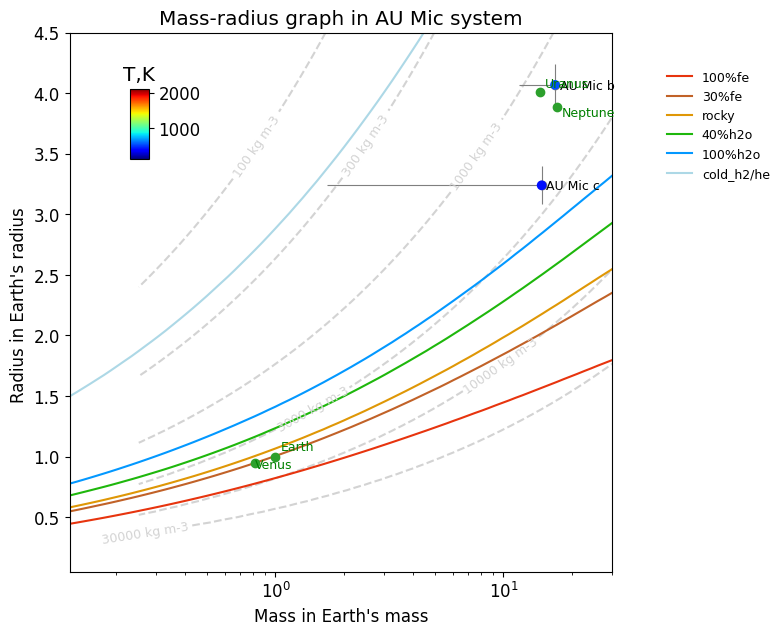
\includegraphics[width=0.45\textwidth]{./img/AU Mic.png}}
    \end{subfigure}
    \hfill
    \begin{subfigure}
        \centering
        \raisebox{-0.5\height}{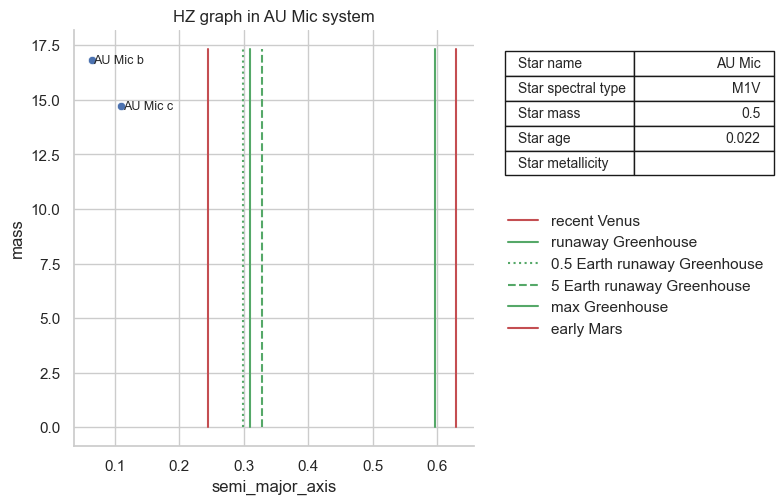
\includegraphics[width=0.45\textwidth]{./img/AU Mic_with_HZ_edges.png}}
    \end{subfigure}
    \caption{AU Mic charts}
    \label{charts-au-mic}
\end{figure}

\begin{figure}[ht!]
    \centering
    \begin{subfigure}
        \centering
        \raisebox{-0.5\height}{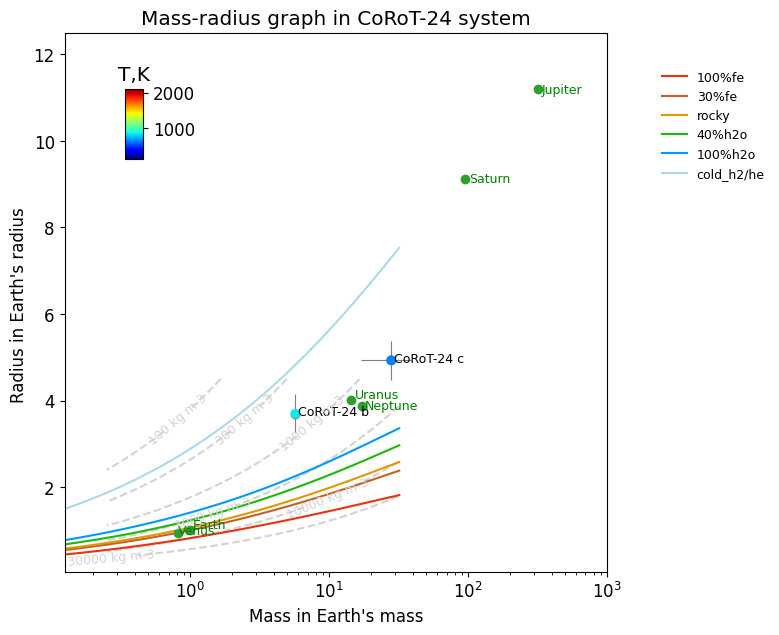
\includegraphics[width=0.45\textwidth]{./img/CoRoT-24.png}}
    \end{subfigure}
    \hfill
    \begin{subfigure}
        \centering
        \raisebox{-0.5\height}{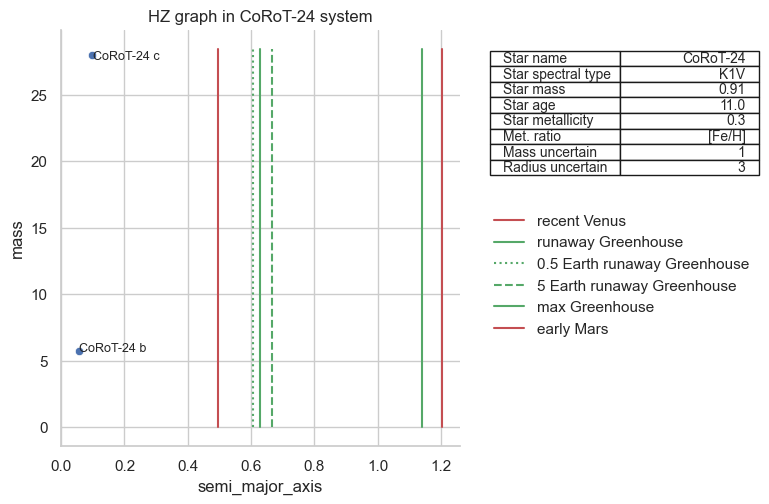
\includegraphics[width=0.45\textwidth]{./img/CoRoT-24_with_HZ_edges.png}}
    \end{subfigure}
    \caption{CoRoT-24 charts}
    \label{charts-corot-24}
\end{figure}

\subsection{Paths}

Using \texttt{[abspath]\{currfile\}}:

\begin{itemize}
    \item absolute path to the current file folder: \currfileabsdir
    \item absolute path to the current file itself: \currfileabspath
\end{itemize}

Using \texttt{\{currfile-abspath\}}:

\begin{itemize}
    \item absolute path to the main file folder: \mainabsdir
    \item absolute path to the main file itself: \mainabspath
\end{itemize}
